% Options for packages loaded elsewhere
\PassOptionsToPackage{unicode}{hyperref}
\PassOptionsToPackage{hyphens}{url}
%
\documentclass[
]{article}
\usepackage{amsmath,amssymb}
\usepackage{lmodern}
\usepackage{iftex}
\ifPDFTeX
  \usepackage[T1]{fontenc}
  \usepackage[utf8]{inputenc}
  \usepackage{textcomp} % provide euro and other symbols
\else % if luatex or xetex
  \usepackage{unicode-math}
  \defaultfontfeatures{Scale=MatchLowercase}
  \defaultfontfeatures[\rmfamily]{Ligatures=TeX,Scale=1}
\fi
% Use upquote if available, for straight quotes in verbatim environments
\IfFileExists{upquote.sty}{\usepackage{upquote}}{}
\IfFileExists{microtype.sty}{% use microtype if available
  \usepackage[]{microtype}
  \UseMicrotypeSet[protrusion]{basicmath} % disable protrusion for tt fonts
}{}
\makeatletter
\@ifundefined{KOMAClassName}{% if non-KOMA class
  \IfFileExists{parskip.sty}{%
    \usepackage{parskip}
  }{% else
    \setlength{\parindent}{0pt}
    \setlength{\parskip}{6pt plus 2pt minus 1pt}}
}{% if KOMA class
  \KOMAoptions{parskip=half}}
\makeatother
\usepackage{xcolor}
\IfFileExists{xurl.sty}{\usepackage{xurl}}{} % add URL line breaks if available
\IfFileExists{bookmark.sty}{\usepackage{bookmark}}{\usepackage{hyperref}}
\hypersetup{
  pdftitle={Exploring the seasonal variation in electric vehicle charging in New Zealand},
  pdfauthor={Pablo Paulsen},
  hidelinks,
  pdfcreator={LaTeX via pandoc}}
\urlstyle{same} % disable monospaced font for URLs
\usepackage[margin=1in]{geometry}
\usepackage{graphicx}
\makeatletter
\def\maxwidth{\ifdim\Gin@nat@width>\linewidth\linewidth\else\Gin@nat@width\fi}
\def\maxheight{\ifdim\Gin@nat@height>\textheight\textheight\else\Gin@nat@height\fi}
\makeatother
% Scale images if necessary, so that they will not overflow the page
% margins by default, and it is still possible to overwrite the defaults
% using explicit options in \includegraphics[width, height, ...]{}
\setkeys{Gin}{width=\maxwidth,height=\maxheight,keepaspectratio}
% Set default figure placement to htbp
\makeatletter
\def\fps@figure{htbp}
\makeatother
\setlength{\emergencystretch}{3em} % prevent overfull lines
\providecommand{\tightlist}{%
  \setlength{\itemsep}{0pt}\setlength{\parskip}{0pt}}
\setcounter{secnumdepth}{-\maxdimen} % remove section numbering
\usepackage{float}
\floatplacement{figure}{H}
\usepackage{comment}
\ifLuaTeX
  \usepackage{selnolig}  % disable illegal ligatures
\fi

\title{Exploring the seasonal variation in electric vehicle charging in
New Zealand}
\author{Pablo Paulsen}
\date{02/18/2022}

\begin{document}
\maketitle

\hypertarget{data-exploration}{%
\subsection{Data Exploration}\label{data-exploration}}

\hypertarget{flip-the-fleet-data-exploration}{%
\subsubsection{Flip the Fleet Data
Exploration}\label{flip-the-fleet-data-exploration}}

Distance traveled and vehicle efficiency (km/kWh) by month, as well as
the region of the vehicle was collected from the on-board computers of
1259 vehicles between 2017 and 2021 as part of the `Flip the Fleet'
project.

A monthly weighted average was calculated for the whole of New Zealand
and then for each region of NZ. The monthly averages were weighted using
the distance traveled to give more weighting to vehicles with higher km
traveled in that month. this was done using the formula
\[\bar{x} = \frac{\sum_{i}^{n} (d_i\times x_i)}{\left(\sum_{i}^{n} d_i\right)\times n}\]

Power consumption (Wh/km) was calculated using the efficiency (km/kWh).
This will be used instead of efficiency in the modeling for reasons that
will become apparent later in the analysis.

\begin{figure}
\centering
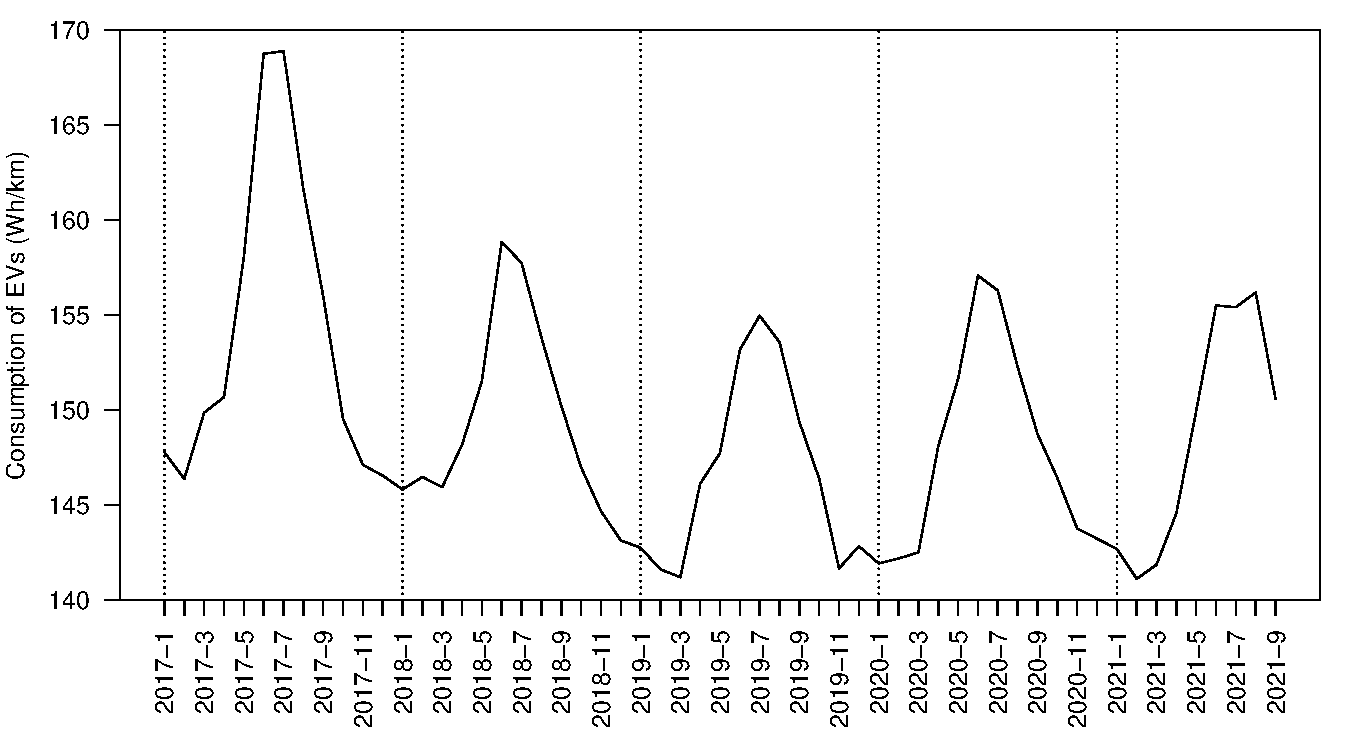
\includegraphics{final_report_files/figure-latex/consum_plot-1.pdf}
\caption{Time series of EVs weighted mean consumption using Flip the
Fleet data from all NZ regions\label{fig:consum_plot}}
\end{figure}

Figure \ref{consum_plot} shows there is a clear seasonal trend in the
monthly average consumption of Flip the Fleets vehicles from all regions
of NZ.

A time series Decomposition is used to isolated the seasonal trend in
consumption from the overall trend. This can be done for all regions of
NZ combined and also for each region independently.

\begin{figure}
\centering
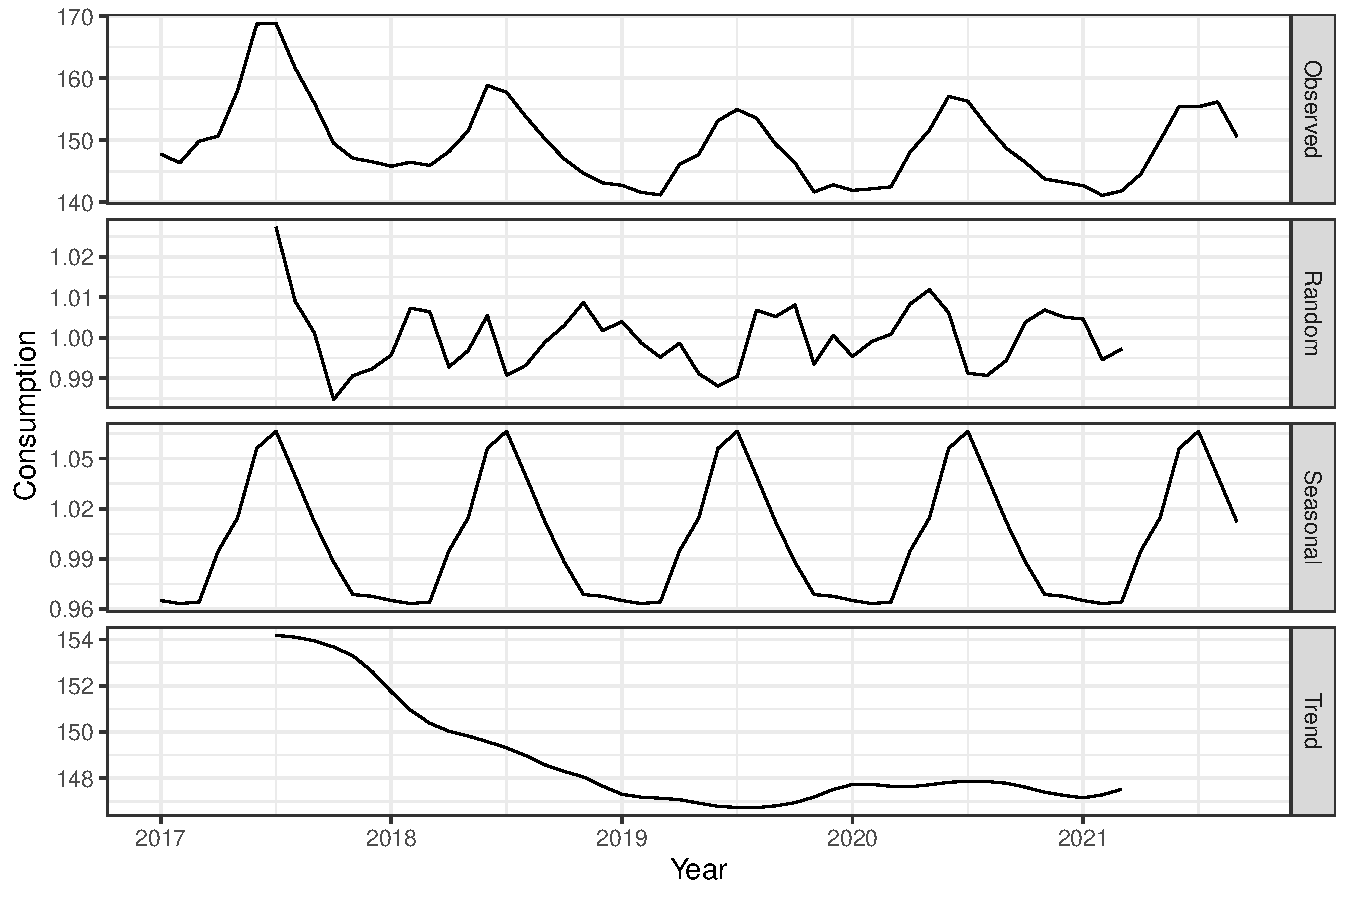
\includegraphics{final_report_files/figure-latex/consum_decomp_plot-1.pdf}
\caption{Multiplicative Time Series Decomposition of Flip the Fleet
Average Consumption for all of NZ\label{fig:consum_decomp_plot}}
\end{figure}

The time series decomposition (Figure \ref{fig:consum_decomp_plot})
shows a very clear seasonal trend. This seasonal trend going from 0.96
times the mean consumption in February to 1.07 times the mean
consumption in February, A peak to peak difference of 10.7\%.

As NZ weather differs significantly by region, to test the hypothesis
that EV consumption is correlated with heating degree days we must limit
the comparison to a single region of Flip the Fleet data and compare it
to that regions weather at the same period of time.

In order to do this hourly weather data from 2017 to 2021 was collected
from the NIWA national climate Database for 14 regions around New
Zealand that best correspond to the regions of the Flip the Fleet
vehicles. The base temperatures were selected to represent the range of
comfortable temperatures for most people, as research shows that a
majority of the seasonal variation in EV efficiency is due to cabin
temperature control\cite{ev_range}. Using the regional hourly
temperatures, monthly heating degree days (HDD) and cooling degree days
(CDD) were imputed using base temperatures of 16\(^\circ\)C and
22\(^\circ\)C respectively. Monthly average temperature was also
calculated.

The HDD and CDD was then divided by the length of the month so that HDD
and CDD corresponds to average heating degrees days per day for the
month. This is so that when comparing to other statistics such as
efficiency that are averaged out rather than summed so there is less
bias.

The calculated monthly weather statistics by region was then added to
the monthly EV data based on the regions of vehicle. This assumes that
vehicle stays in it's own region for a majority of the time.

\begin{figure}
\centering
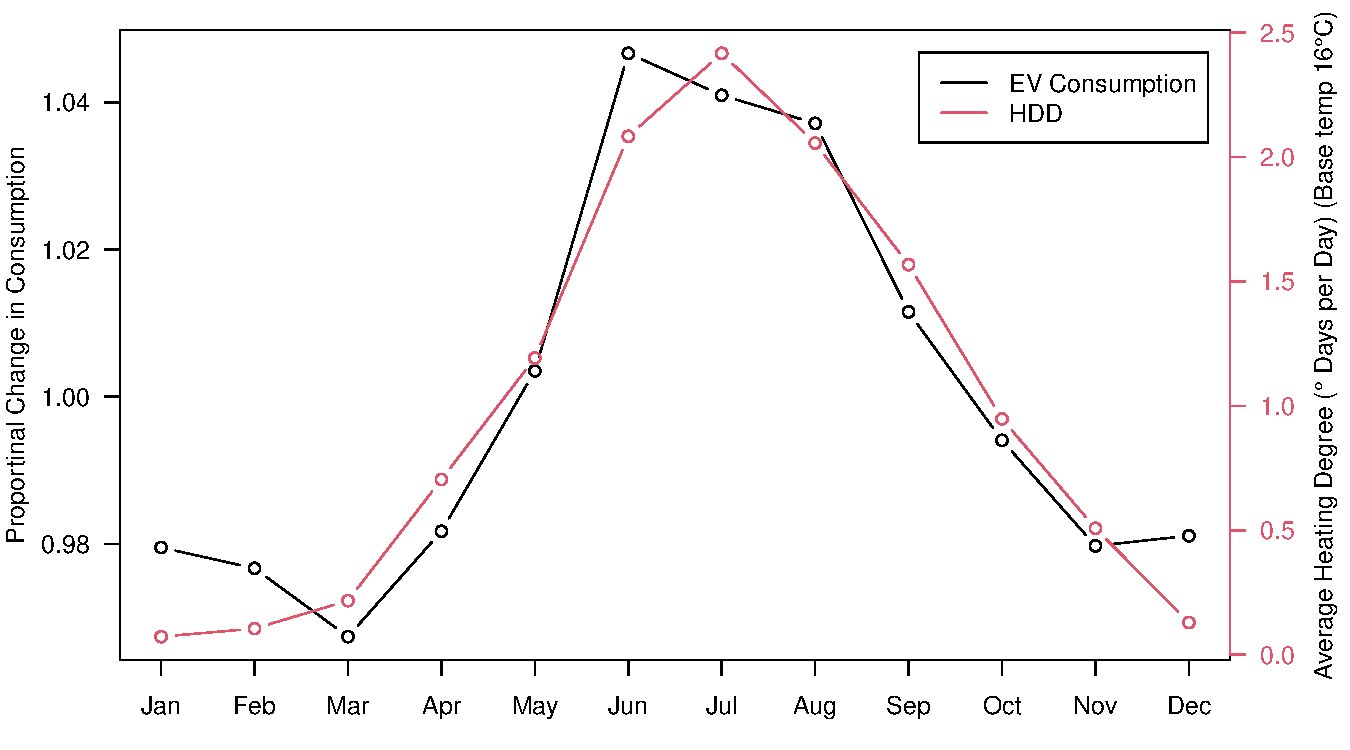
\includegraphics{final_report_files/figure-latex/consum_HDD_plot-1.pdf}
\caption{Auckland seasonal HDD and EV Consumption
decompostions\label{fig:consum_HDD_plot}}
\end{figure}

Auckland is used as an example to compare correlation between HDD and
consumption as it has the largest amount of data and is of most interest
to Vector. Within Auckland Figure \ref{fig:consum_HDD_plot} shows very
clearly that HDD and consumption of EVs are highly correlated. There is
a slight increase in consumption in January and February and it can be
questioned if that is due to AC usage which would decrease range
\cite{ev_range} or other factors such as holiday travel which could
involve highway driving which EVs are generally less efficient at
\cite{ev_highway}. This effect is not obvious in the overall trend this
could be as Auckland for the most part is a warmer climate than the rest
of NZ.

\begin{figure}
\centering
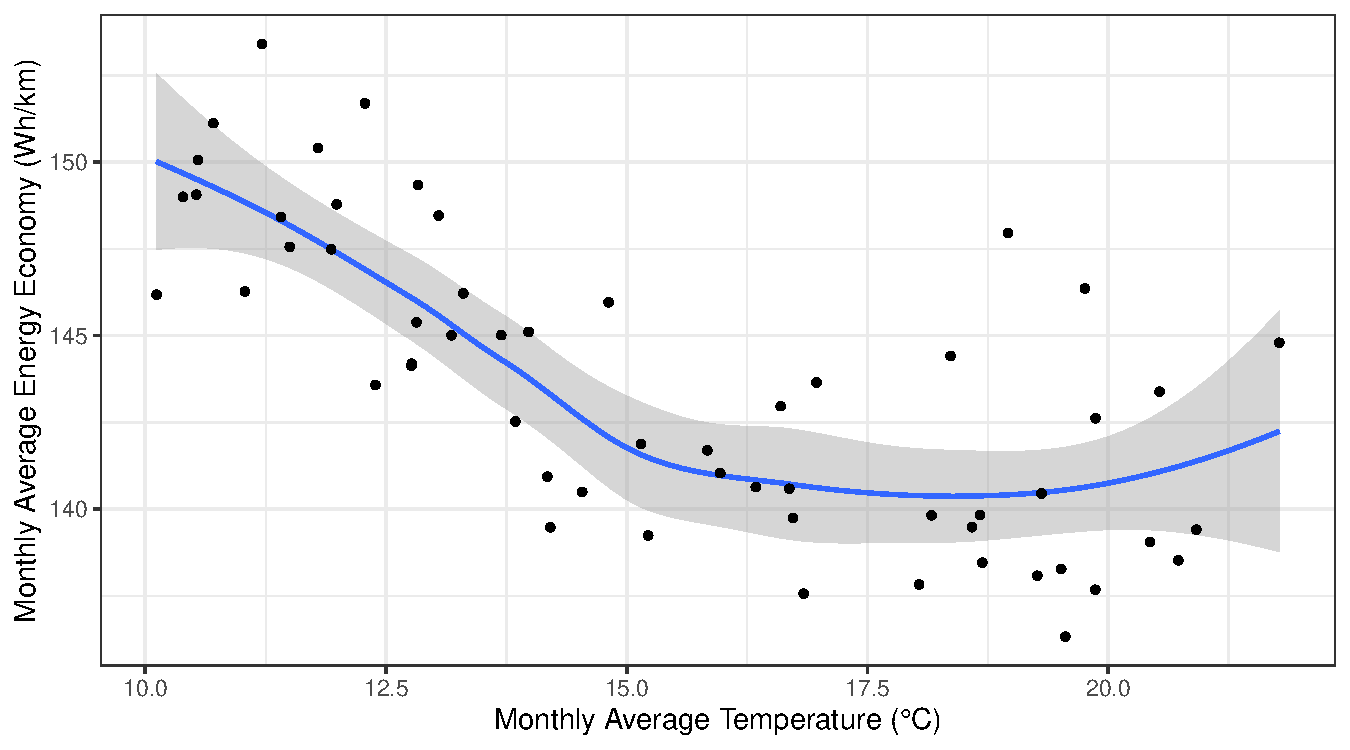
\includegraphics{final_report_files/figure-latex/temp_consum_plot-1.pdf}
\caption{Auckland monthly average consumption by avg
temperature\label{fig:temp_consum_plot}}
\end{figure}

Further looking into Auckland consumption by weather Figure
\ref{fig:temp_consum_plot} shows a decreasing consumption up to around a
monthly average temperature of 17.5°C. However, increasing monthly
average temperature past this there appears to be a trend towards
increasing EV consumption.As stated previously research \cite{ev_range}
suggested AC also increases consumption of the EV. This suggest it may
be worth including cooling degree days and heating degree days in
analysis. This could also be useful to explain the points well above the
trend line that may be from a month where there was both cold and warm
days contributing to a high usage of cabin temperature control
increasing consumption but average temperature would not be able to show
this.

\hypertarget{nz-vkt-data-exploration}{%
\subsubsection{NZ VKT Data Exploration}\label{nz-vkt-data-exploration}}

If we know EV consumption has a seasonal trend in order to see how this
will affect the grid we need to see how this correlates with NZ
populations driving pattern.

To find if a seasonal trend in fuel usage in NZ fuel trade data
\cite{fuel_trade} from the Ministry of Business, Innovation and
Employment (MBIE) is used. This data set quarterly data in broken down
by fuel type and sector. This allows the isolation of petrol usage in
domestic land transport which should be an accurate representation of
the fuel usage by light passenger vehicles.

\begin{figure}
\centering
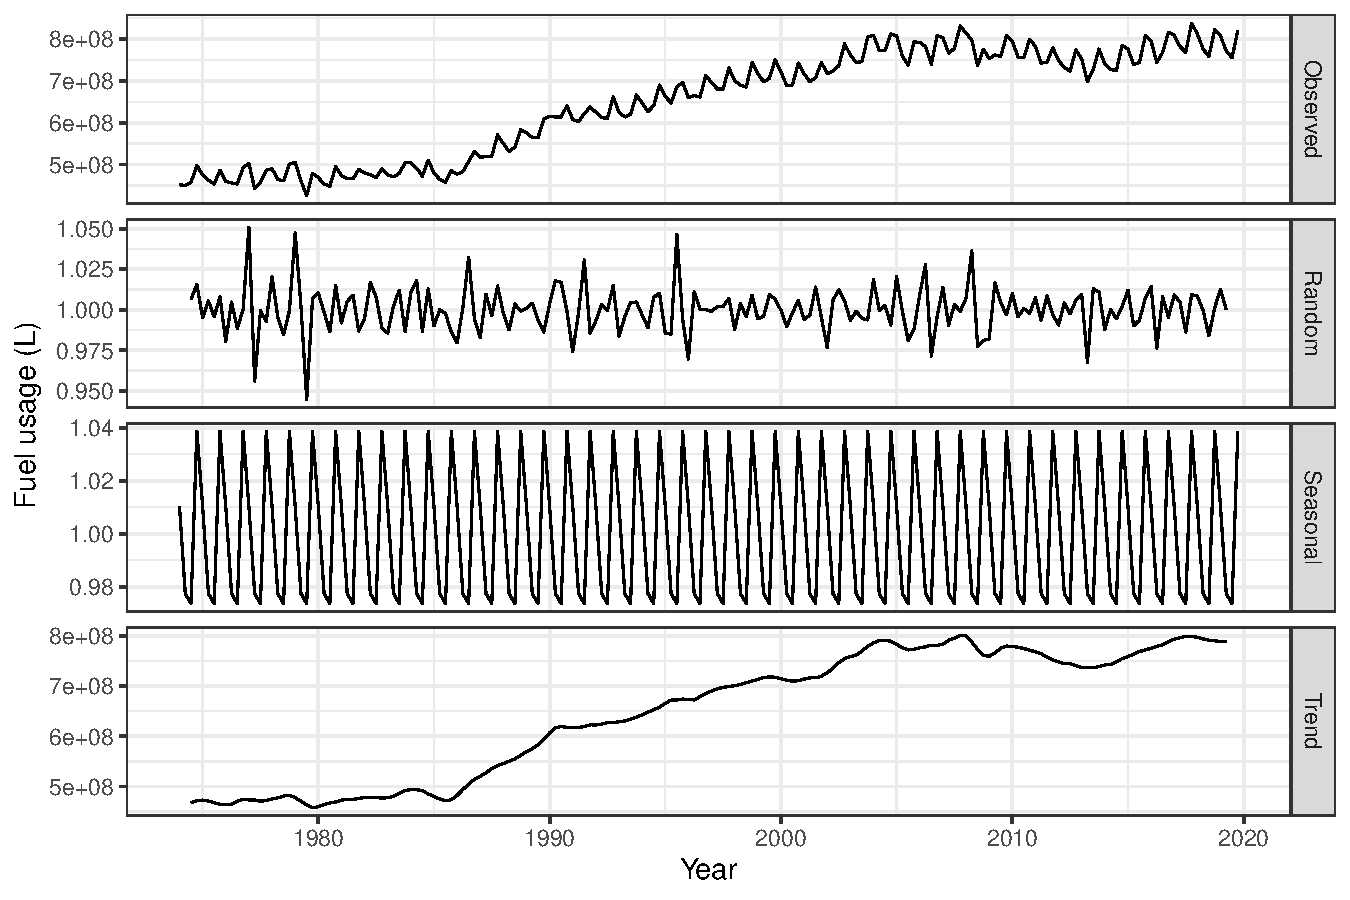
\includegraphics{final_report_files/figure-latex/petrol_ts-1.pdf}
\caption{Decomposition of Multiplicative Petrol Usage Time Series}
\end{figure}

\hypertarget{model}{%
\subsection{Model}\label{model}}

\begin{thebibliography}{9}
\bibitem{ev_range}
\textit{To what degree does temperature impact EV range?}
\\\texttt{\url{https://www.geotab.com/blog/ev-range/}}
\bibitem{ev_highway}
\textit{Why is the range of an EV less on the freeway than the city?}
\\\texttt{\url{https://evcentral.com.au/why-is-the-range-of-an-ev-less-on-the-freeway-than-the-city/}}
\bibitem{fuel_trade}
\textit{MBIE oil trade statistics}
\\\texttt{\url{https://www.mbie.govt.nz/building-and-energy/energy-and-natural-resources/energy-statistics-and-modelling/energy-statistics/oil-statistics/}}
\bibitem{HDD_est}
\textit{Bayesian estimation of a building's base temperature for the calculation of heating degree-days}
\\\texttt{\url{https://www.sciencedirect.com/science/article/abs/pii/S0378778816312907}}
\bibitem{NZTA_VKT}
\textit{NZTA VKT data website}
\\\texttt{\url{https://www.transport.govt.nz/statistics-and-insights/fleet-statistics/vehicle-kms-travelled-vkt-2/}}
\bibitem{times_model}
\textit{ECCA Times Model}
\\\texttt{\url{https://www.eeca.govt.nz/insights/data-tools/new-zealand-energy-scenarios-times-nz/}}
\end{thebibliography}

\end{document}
